\documentclass[bibliography=totoc,captions=tableheading,titlepage=firstiscover]{scrartcl}

\usepackage{scrhack}

\usepackage[aux]{rerunfilecheck}

\usepackage{polyglossia}
\setmainlanguage{german}

\usepackage[backend=biber,]{biblatex}
\addbibresource{lit.bib}
\usepackage{amsmath}
\usepackage{amssymb}
\usepackage{mathtools}

\usepackage{fontspec}

\usepackage[
  math-style=ISO,
  bold-style=ISO,
  sans-style=italic,
  nabla=upright,
  partial=upright,
]{unicode-math}

\usepackage[
  locale=DE,
  separate-uncertainty=true,
  per-mode=reciprocal,
  output-decimal-marker={,},
]{siunitx}

\usepackage{float}
\floatplacement{figure}{htbp}
\floatplacement{table}{htbp}

\usepackage[
  labelfont=bf,
  font=small,
  width=0.9\textwidth,
]{caption}

\usepackage{graphicx}
\usepackage{grffile}

\usepackage{booktabs}

\usepackage[
  unicode,
]{hyperref}

\usepackage{bookmark}

\begin{document}
  \section{Ziel des Versuchs}
  Der Versuch zielt auf eine präzise Messung der Brechungindizes von Luft und eines gläsernen Plättchens unter Verwendung eines Sagnac-Interferometers ab.

  \section{Theorie}
  Das verwendete Interferometer, benannt nach Georges Sagnac, nutzt den Effekt der Interferenz zur präzisen Messung von unterschieden in der optischen Dichte verschiedener Materialien. Da zur Intereferenz zwei unterschiedliche optische Signale benötigt werden, teilt ein sogenannter polarizing beam-splitting Cubes (PBSC) den zur Untersuchung verwendeten Laserstrahl. Hierbei handelt es sich um einen durchsichtigen Würfel, welcher aus zwei Prismen zusammengesetzt ist. Die in seinem Inneren auftretende Grenzfläche sorgt für eine teilweise Reflexion des einfallenden Strahles und eine teilweise Transmission. Es treten folglich zwei Strahlen in zwei senkrecht zueinander stehende Richtungen aus dem PBSC aus. Zusätzlich sind diese Strahlen zueinander orthogonal polarisiert, d.h. es kann keine Interferenz zwischen beiden Strahlen auftreten. Dementsprecend müssen beide Strahlen vor der Detektion z.B. durch einen Polarisationsfilter auf eine gemeinsame Achse projiziert werden. Da der PBSC jedoch lediglich die im einfallenden Strahl überlagerten Polarisationen auseinanderfiltert muss der einfallende Strahl um 45\circ gegen die Vertikale gekippt polarisiert sein, um eine gleiche Intensität der beiden Teilstrahlen zu gewährleisten. Diese beiden STrahlen durchlauden im Interferometer einen nur geringfügig versetzten Weg, also im Gegensatz zum Michelson-Interferometer die gleichen Spiegel. Sie werden im gleichen PBSC getrennt und, nach einem geschlossenen Umlauf durchs Interferometer, wieder überlagert. Dies bildet ein sehr präzises Messgerät, da bspw. kleine Produktionsunterschiede der Spiegel (z.B. unterschiedlich dickes GLas) nicht zu Unterschieden in den Strahlengängen fährt. Die Qualität von Interferometern wird durch den Kontrast $K$ bestimmt. Es gilt:
  \begin{equation}
  	\label{eq:kontrast}
	K = \frac{I_{max}+I_{min}}{I_{max}+I_{min}}
  \end{equation}
Hierbei bezeichnet $I_{max}$ die Intensität der Interferenzmaxima, $I_{min}$ entsprechend die der Interferenzminima. Diese Intensität hängt stark von der Polarisation des Ursprungsstrahls ab, da gilt: $I~<|E_h+E_v|^2>$ und die $E$-Feld Komponenten naturgemäß abhängig sind vom Winkel des Ursprungsstrahls $E = E_0 \cos (\omega t)$ gegen die Vertikale. O.B.d.A. wird der im Interferometer verursachte Gangunterschied $\delta$ zwischen den beiden Komponenten als Unterschied der horizontalen gegen die Vertikale betrachtet. So ergibt sich
\begin{equation}
	K_v = E_0 \cos (\phi) \cos(\omega t)
\end{equation}
sowie
\begin{equation}
	K_h = E_0 \sin(\phi) \cos(\omega t + \delta)
\end{equation}
mit $\phi$ als Polarisationswinkel. Die Intensität lässt sich somit durch
\begin{align*}
	I ~ <|E_h+E_v|^2> &=<| E_0 \cos (\phi) \cos(\omega t) +  E_0 \sin(\phi) \cos(\omega t + \delta)|^2> \\
			       %&= < E_0^2 \cos(\phi)^2 \cos(\omega t)^2 +2E_0^2 \cos(\phi) \sin(phi) \cos(\omega t) \cos(\omega t + \delta) + E_0^2 \sin(\phi)^2 \cos(\omega t +\delta)^2 \\
			       %&= E_0^2 \cos(\phi)^2 <\cos(\omega t)^2> + 2 E_0^2 \cos(\phi) \sin(\phi) <\cos(\omega t) \cos(\omega t + \delta> + E_0^2 \sin(\phi)^2 <\cos(\omega t+ \delta)^2> \\
			       &= \frac{E_0^2}{2} \pm E_0^2 \cos(\phi)\sin(\phi)
\end{align*}
Da nur konstruktive, bzw destruktive, Interferenz betrachtet wird, gilt $\delta = 2\pi n$, mit $n \in \mathbb{N}$, bzw. $\delta = (2n+1)\pi$, mit $n \in \mathbb{N}$, was zu $\pm$-Unterscheidung führt. Zudem gilt allgemein $<\cos(\omega t + \delta)> = \frac{1}{2}$.
Durch Vernachlässigung aller Vorfaktoren ergibt sich für die Proportionalität von $K$
\begin{equation}
	K ~ \cos(\phi)\sin(\phi)
\end{equation}
Ist dieser Kontrast hinreichend groß, kann eine zuverlässige Bestimmung der Druckabhängigkeit der Brechungszahl eines optisch dünnen Gases, bzw. Gemisches, erfolgen, indem in einen Strahl eine Gaszelle der Länge L eingebracht wird. In dieser wird der Druck von $p_1$ auf $p_2$ variiert und die Anzahl $M$ der dabei auftretenden Interferenzmaxima gemessen. Hierfür gilt die Formel

\begin{equation}
	M = \frac{\Delta n}{\lambda_{vac}} L
\end{equation}
bei der $\lambda_{vac}$ die Wellenlänge des Lasers bezeichnet.
Der Brechungsindex $n_0$ bei $T_0 = \SI{273,15}{\kelvin}$ und $p_0 =  \SI{1013,2}{\milli\bar}$ ergibt sich nach \cite{Anleitung} über
\begin{equation}
	n(p_0,T_0)=1+ \Delta n \frac{T}{T_0} \frac{p_0}{p_2-p_1}.
	\label{eqn:n0}
\end{equation}

Zur Messung des Brechungsindex eines Plättchens wird eine Halterung mit zwei um $\Phi = 20\circ$ gegeneinander geneigte Plättchen verwendet. Jeder der beiden Strahlen durchläuft eines der beiden Plättchen und erhält damit, einmal durch den durch Brechung verlängerten Weg, einmal durch den geänderten Brechungsindex eine Phasenverschiebung. Werden die Plättchen in der optischen Ebene um $\theta$ gedreht, detektiert man wieder Interfenzmaxima $M$.
Für eine die Platten gilt näherungsweise für kleine Winkel
\begin{equation}
	M = (n-1)\frac{T}{\lambda_{vac}}(1+\frac{\theta^2-\Phi^2}{2n}.
  \label{eq:index}
\end{equation}

Der Brechungsindex lässt sich dann über
\begin{equation}
	n = \frac{2\Phi \theta T}{2\Phi \theta T-M \lambda_{vac}}.
\end{equation}

	\section{Durchführung}

  \begin{figure}[H]
    \center
    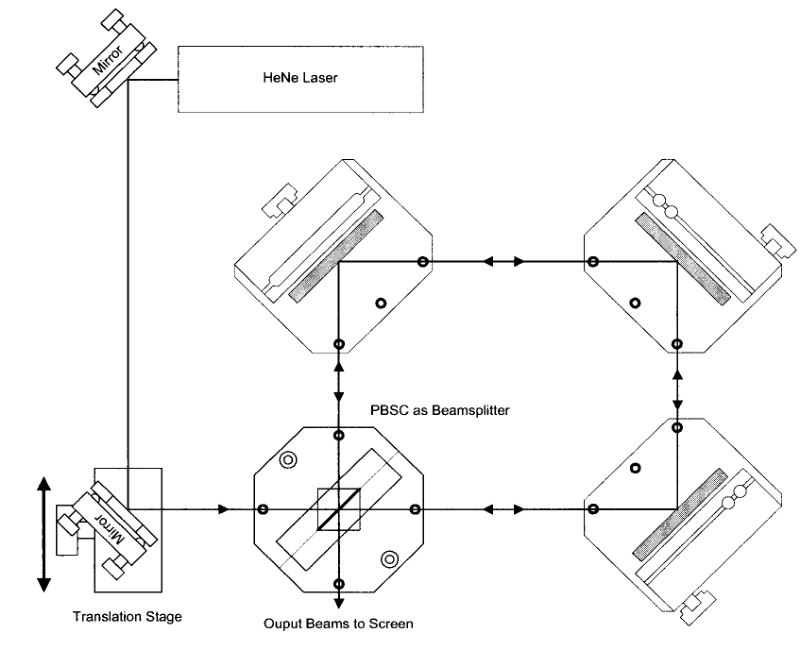
\includegraphics[width=\textwidth]{Versuchsaufbau.JPG}
    \label{fig:aufbau}
    \caption{Aufbau des Sagnac-Interferometers}
  \end{figure}
  \begin{figure}[H]
    \center
    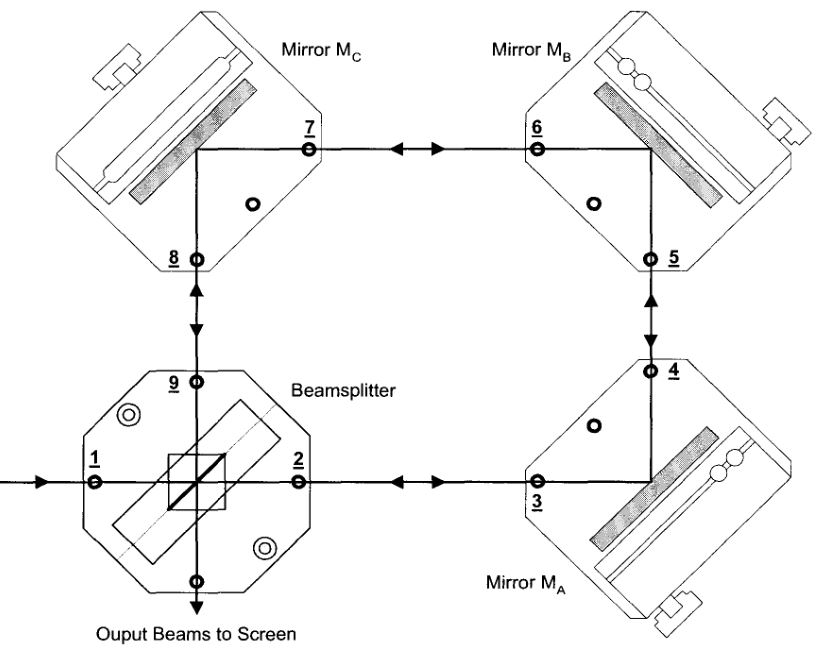
\includegraphics[width=\textwidth]{Strahlengang.JPG}
    \label{fig:bauteilpos}
    \caption{Strahlengang des Sagnac-Interferometers und Montagepunkte der Lochblenden zur Justage}
  \end{figure}
  In den Abbildungen \ref{fig:aufbau} und \ref{fig:bauteilpos} ist der generelle Aufbau des Sagnac Interferometers zu sehen. Hinter dem PBSC aus der Abbildung wird
  zur Messung der Interferenzmuster noch ein weiterer PBSC zur Teilung des Strahls auf 2 Photodioden eingebaut. Die Signale der Dioden werden auf einem Oszilloskop von einander subtrahiert und
  als Differenzsignal visualisiert.
  Zur zusätzlichen Justierung wird der HeNe-Laserstrahl vor dem Auftreffen auf den PBSC noch über 2 Spiegel geleitet. Durch den linken unteren Spiegel kann die Aufteilung des Strahls in hin- und rückläufigen
  Strahl bewirkt werden, was für die späteren Messungen von nöten ist. Zur korrekten Justierung des Strahls auf die Spiegel werden ausserdem Lochblenden verwendet.\\
  Bevor mit der Messung der Intensitätsmaxima und Minima begonnen werden kann, werden nun die die Strahlen im Interferometer korrekt auf die Photodiode
  ausgerichtet.\\
  Anschließend werden die Plättchen in das Interferometer gebracht. Nun wird der Polarisationsfilter, welcher vor Punkt 1 positioniert ist,
  in 10\circ Schritten gedreht. Aus dem auf dem Oszilloskop sichtbaren Referenzsignal lassen sich nun die maximalen und minimalen Intensitäten ablesen, welche entstehen, wenn
  man die Plättchen im Interferometer um einen Winkel im Strahl kippt. Aus den gemessenen Daten wird in der Auswertung der Kontrast errechnet.\\
  \\
  Im zweiten Teil des Versuchs soll der Brechungsindex der zuvor bereits verwendeten Plättchen ermittelt werden. Dazu werden die um 10\circ aus der Ebene senkrecht zum Strahl gekippten Plättchen in Laserstrahl des Interferometers eingeführt.
  Anschließend wird die Anzahl der Interferenzmaxima bei einer Rotation um 10 - 11 Grad senkrecht zur Strahlebene in 1 Grad Schritten gemessen.\\
  \\
  Im letzten Teil des Versuchs wird statt der Plättchen eine Gaszelle in den Laserstrahl geschoben und mithilfe einer angeschlossenen Vakuumpumpe evakuiert.
  Hier werden die Anzahl der Counts bei zurück auf Umgebungsdruck steigendem Druck in der Kammer aufgenommen.
\section{Auswertung}
\subsection{Messung des Kontrasts der Apparatur}
Für die Ermittlung des Kontrasts des Interferometer wird ein Laser mit einer Wellenlänge von $\lambda_{vac}=\SI{623.99}{\nano\meter}$ verwendet.
Aus den gemessenen Intensitäten wird dann mithilfe von Formel \eqref{eq:kontrast} der Kontrast berechnet.
Die Messwerte, sowie der berechnete Kontrast sind in Tabelle \ref{tab:Kontrast} zusammengestellt.
Das Maximum des Kontrasts liegt bei einem Winkel von 60\circ.\\
\begin{figure}[H]
  \center
  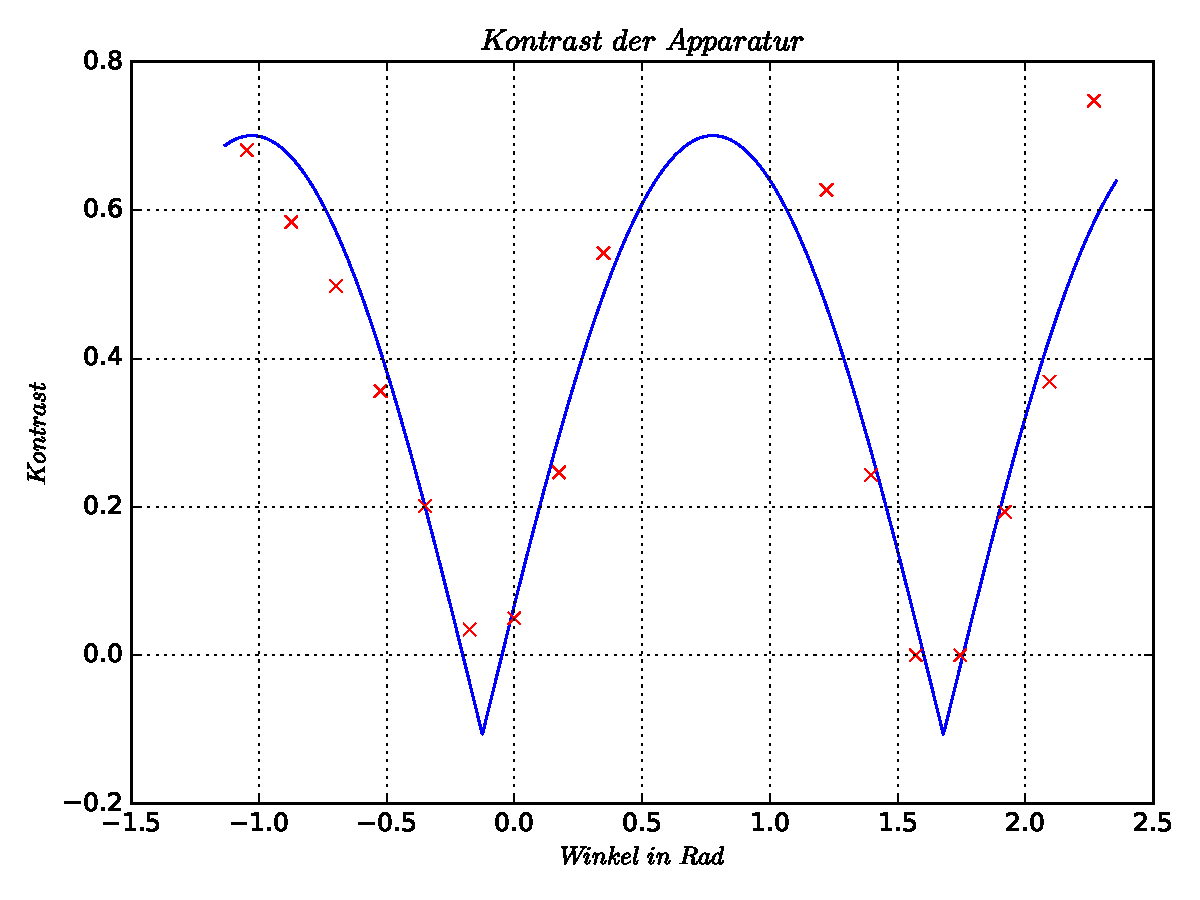
\includegraphics[width=0.65\textwidth]{kontrastplot.pdf}
  \caption{Winkel der Platten und aus den gemessenen Intensitäten errechneter Kontrast.}
  \label{fig:kontrastplot}
\end{figure}
\begin{table}[H]
  \center
  \caption{Zu unterschiedlichen Winkeln gemessene Intensitäten dazu errechneter Kontrast.}
  \label{tab:Kontrast}
\begin{tabular}{c|c|c|c}
  Winkel in Grad& $U_{min}$ in mV& $U_{max}$ in mV& Kontrast\\
  \hline
  -60 &    -1085&       25& 0.6808\\
  -50 &     -975&       25& 0.5841\\
  -40 &  -969.75&   -37.50& 0.4979\\
  -30 &  -969.75&  -281.25& 0.3561\\
  -20 & -1118.75& -1012.50& 0.2013\\
  -10 & -1106.75&  -668.75& 0.0347\\
  0   & -1118.75& -1043.75& 0.0498\\
  10  & -1118.75&  -743.75& 0.2465\\
  20  & -1118.75&  -531.25& 0.5422\\
  30  & -1118.75&  -375.00& 0.9255\\
  40  & -1118.75&  -293.75& 0.95\\
  45  & -1118.75&  -212.50& 0.955\\
  50  & -1118.75&   -87.50& 0.8549\\
  \hline
  60  & -1118.75&   -18.75& 0.9670\\
  \hline
  70  & -1118.75&  -256.25& 0.6273\\
  80  & -1118.75&  -681.25& 0.2431\\
  90  &        -&        -&      0\\
  100 &        -&        -&      0\\
  110 & -1118.75&  -756.25& 0.1933\\
  120 &  -1125.0&  -518.75& 0.3688\\
  130 &  -1125.0&  -162.50& 0.7476\\
\end{tabular}
\end{table}
In \ref{fig:kontrastplot} ist der Kontrast in Abhängigkeit des Drehwinkels der Platten aufgetragen und mithilfe von $curve-fit$ gefitted worden.
Um die Messwerte optimal durch einen Fit zu approximieren wurden die Messwerte zwischen $30^\circ$ und $60^\circ$ aus dem Diagramm entfernt. Bei $90^\circ$ und $100^\circ$ sind beide Intensitäten im Hintergrundrauschen untergegangen, woraus sich der Kontrast von 0 ergibt.\\
\subsection{Berechnung des Brechungsindex der Platten}
  In der Anleitung \cite{Anleitung} finden sich zur Berechnung des Brechungsindex der Platten folgende Herstellerangaben:\\
\begin{center}
  $T = \SI{1}{\milli\meter}$, $n_{\symup{Lit}}=1.35$, $\delta =10$\circ
\end{center}
Anhand dieser Angaben, sowie den gemessenen Werten, wird mithilfe von Formel \eqref{eq:index} aus der Theorie der Brechungsindex der Platten errechnet.
Die berechneten Werte sind in Tabelle \ref{tab:plattenindex} einzusehen.\\
\begin{table}[H]
  \center
  \caption{Gemessene Counts bei einer Drehung der Platten um ca. $\theta=10^\circ$ und Mittelwert des berechneten Brechungsindex.}
	\label{tab:plattenindex}
  \begin{tabular}{c|c|c|c}
    Messung& Counts M& Brechungsindex n& Fehler\\
    \hline
    1& 55& 1.049& 0.036\\
    2& 40& 1.038& 0.027\\
    3& 55& 0.750& 1.159\\%Bullshit messung! in den messwerten ist auch n fetter sprung.
    4& 51& 1.015& 0.050\\
    5& 55& 1.015& 0.054\\
    6& 43& 1.036& 0.031\\
    7& 37& 1.023& 0.023\\
    8& 34& 1.034& 0.023\\
  \end{tabular}
\end{table}
\subsection{Berechnung des Brechungsindex von Luft}
In den Tabellen \ref{tab:druckdaten1} und \ref{tab:druckdaten2} sind die mithilfe von Formel \eqref{eq:luft} berechneten Werte des Brechungsindex von Luft bei steigendem Druck zu sehen.
Die Wellenlänge des Lasers beträgt nach wie vor $\lambda_{vac}=\SI{632.99}{\nano\meter}$. Die Länge der Gaszelle ist durch $L=\SI{10}{\centi\meter}$ gegeben.
\begin{table}[H]
  \center
  \caption{Brechungsindex von Luft bei steigendem Druck in 100 mbar Schritten.}
  \label{tab:druckdaten1}
 \begin{tabular}{c|c|c|c}
   $p_1$ in mbar&$n_1$ &$p_2$ in mbar &$n_2$\\
   \hline
   11  &1.000 070 & 12  & 1.000 076\\
   100 &1.000 633 & 100 & 1.000 633\\
   200 &1.001 266 & 200 & 1.001 266\\
   300 &1.001 899 & 300 & 1.001 899\\
   400 &1.002 532 & 400 & 1.002 532\\
   500 &1.003 165 & 500 & 1.003 165\\
   600 &1.003 798 & 600 & 1.003 798\\
   700 &1.004 431 & 700 & 1.004 431\\
   800 &1.005 064 & 800 & 1.005 064\\
   900 &1.005 697 & 900 & 1.005 697\\
   995 &1.006 298 & 995 & 1.006 298\\
 \end{tabular}
\end{table}
\begin{table}[H]
    \center
    \caption{Brechungsindex von Luft bei steigendem Druck in 50 mbar Schritten.}
    \label{tab:druckdaten2}
    \begin{tabular}{c|c|c|c}
      $p_3$ in mbar&$n_3$ &$p_4$ in mbar &$n_4$\\
      \hline
      8  & 1.000 051& 8  & 1.000 051\\
      50 & 1.000 317& 50 & 1.000 317\\
      100& 1.000 633& 100& 1.000 633\\
      150& 1.000 949& 150& 1.000 949\\
      200& 1.001 266& 200& 1.001 266\\
      250& 1.001 582& 250& 1.001 582\\
      300& 1.001 899& 300& 1.001 899\\
      350& 1.002 215& 350& 1.002 215\\
      400& 1.002 532& 400& 1.002 320\\
      450& 1.002 848& 450& 1.002 848\\
      500& 1.003 165& 500& 1.003 165\\
      550& 1.003 481& 550& 1.003 481\\
      600& 1.003 798& 600& 1.003 798\\
      650& 1.004 114& 650& 1.004 114\\
      700& 1.004 431& 700& 1.004 431\\
      750& 1.004 747& 750& 1.004 747\\
      800& 1.005 064& 800& 1.005 064\\
      850& 1.005 380& 850& 1.005 380\\
      900& 1.005 697& 900& 1.005 697\\
      950& 1.006 013& 950& 1.006 013\\
      995& 1.006 298& 995& 1.006 298\\
    \end{tabular}
\end{table}

\section{Diskussion}
Offensichtlich sind die starken Schwankungen bei der Messung des Brechungindexes der Glasplatten zwischen $0,7590$ und $1.034$ \ref{tab:plattenindex}, sowie deren dramatische Abweichung vom Theoriewert von $1,35$. Vernachlässigt man den stark aus der Reihe fallenden Wert von $0,75$, welcher vermutlich Erschütterungen des Interferometers geschuldet ist, so bleibt dennoch die Abweichung von $n_1$ vom Theoriewert in drei Größenordnungen.

Die Messung des Brechungindexes von Luft ergibt mit konstant $1.006298$ bei $\SI{995}{\milli\bar}$ solide Ergebnisse.

\printbibliography
\nocite{*}
\end{document}
